\documentclass[11pt]{article}
\usepackage[margin=0.78in]{geometry}
\usepackage{amsmath,amssymb,bm,booktabs,array}
\usepackage{xcolor,graphicx,tikz}
\usetikzlibrary{arrows.meta,positioning}
\usepackage[most]{tcolorbox}
\usepackage{enumitem,fancyhdr,hyperref,microtype}
\graphicspath{{results/aescte_dsmc/}}
\definecolor{navy}{HTML}{17365D}
\definecolor{blue}{HTML}{2F75B5}
\definecolor{teal}{HTML}{2A9D8F}
\definecolor{gold}{HTML}{E9A23B}
\definecolor{red}{HTML}{C44536}
\definecolor{lightblue}{HTML}{EAF3F8}
\definecolor{lightgold}{HTML}{FFF6E6}
\hypersetup{colorlinks=true,linkcolor=navy,urlcolor=blue,citecolor=navy}
\pagestyle{fancy}\fancyhf{}
\lhead{M\&I-ENG 690A -- AI in Fluid Mechanics}\rhead{Week 10 Extension}\cfoot{\thepage}
\setlength{\headheight}{14pt}
\setlist{itemsep=3pt,topsep=4pt}
\newtcolorbox{learningbox}{colback=lightblue,colframe=blue,title=Learning checkpoint,fonttitle=\bfseries}
\newtcolorbox{warningbox}{colback=lightgold,colframe=gold,title=Scientific boundary,fonttitle=\bfseries}
\newtcolorbox{evidencebox}{colback=white,colframe=navy,title=Evidence gate,fonttitle=\bfseries}
\newtcolorbox{decisionbox}{colback=teal!6,colframe=teal,title=Decision rule,fonttitle=\bfseries}
\newcommand{\Kn}{\mathrm{Kn}}
\newcommand{\RelLtwo}{\varepsilon_{L_2}}

\begin{document}
\hypersetup{pageanchor=false}
\begin{titlepage}
\centering\vspace*{0.75cm}
{\color{navy}\rule{\textwidth}{2pt}}\\[0.45cm]
{\Huge\bfseries DSMC Data-Driven Surrogates\\[0.16cm]from Particles to Reproducible Fields\par}
\vspace{0.32cm}{\Large Rarefied cavity, monatomic shock, and diatomic relaxation\par}
\vspace{0.32cm}{\large Week 10 Extension Lecture Notes\par}
\vspace{0.48cm}{\color{navy}\rule{\textwidth}{2pt}}\\[0.8cm]
{\Large M\&I-ENG 690A -- AI in Fluid Mechanics\par}
\vspace{0.2cm}{\large Summer 2026\par}
\vfill
\begin{tcolorbox}[colback=lightblue,colframe=blue,width=0.92\textwidth]
\textbf{Central question.} How do we qualify noisy particle-solver fields as
numerical evidence, then reproduce cavity and shock surrogates without hiding
the physical case definition, the assessment metric, or an unavailable target?
\end{tcolorbox}
\vfill{\large Instructor: Ehsan Roohi\par}
\end{titlepage}

\hypersetup{pageanchor=true}
\pagenumbering{roman}\tableofcontents\newpage\pagenumbering{arabic}

\section{Learning Contract and Evidence Map}
This lecture accompanies the executable Week 10 notebook and the article by
Roohi and Shoja-Sani, \emph{Data-driven surrogate modeling of DSMC solutions
using deep neural networks}, Aerospace Science and Technology 168 (2026)
110785, DOI \href{https://doi.org/10.1016/j.ast.2025.110785}{10.1016/j.ast.2025.110785}.

\begin{learningbox}
By the end of the lecture, a student should be able to:
\begin{enumerate}
\item summarize the DSMC move--collide--sample cycle;
\item specify mesh, time-step, particle, sampling, and conservation checks;
\item parse a complete numerical field and verify its provenance;
\item derive the log-$\Kn$ cavity synthesis used in the article;
\item build a POD-trunk/parameter-branch shock operator;
\item compare interpolation and one-sided extrapolation; and
\item regenerate every retained metric and figure from committed tables.
\end{enumerate}
\end{learningbox}

\begin{center}
\begin{tabular}{p{0.23\textwidth}p{0.35\textwidth}p{0.31\textwidth}}
\toprule
Evidence layer & Question & Retained artifact \\
\midrule
Raw DSMC & What was actually computed? & 85 source files, units, grids, run metadata \\
Data contract & Did parsing preserve the cases? & SHA-256 manifest and shape checks \\
Surrogate & Does the map predict a complete unseen case? & field/profile errors and contours \\
Course release & Can another student rerun it? & notebook, CLI scripts, tests, lecture PDF \\
\bottomrule
\end{tabular}
\end{center}

\clearpage
\section{DSMC as an Independent Numerical Solver}
For a dilute gas, $\Kn=\lambda/L$ measures the molecular mean free path
$\lambda$ relative to a characteristic length $L$. DSMC represents many real
molecules by simulation particles and advances them through a statistically
equivalent kinetic experiment.

\subsection{One DSMC time step}
\begin{center}
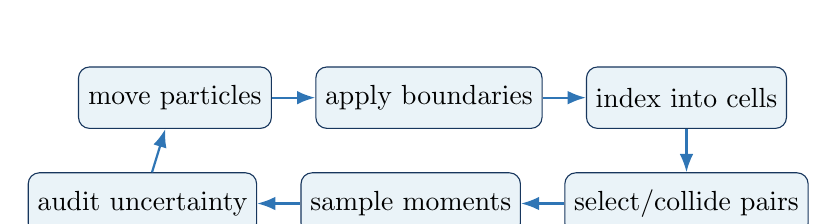
\begin{tikzpicture}[node distance=0.55cm and 0.55cm,>=Latex]
\tikzset{box/.style={draw=navy,rounded corners,minimum width=2.45cm,minimum height=0.78cm,align=center,fill=lightblue}}
\node[box] (move) {move particles};
\node[box,right=of move] (bound) {apply boundaries};
\node[box,right=of bound] (index) {index into cells};
\node[box,below=of index] (collide) {select/collide pairs};
\node[box,left=of collide] (sample) {sample moments};
\node[box,left=of sample] (audit) {audit uncertainty};
\draw[->,thick,blue] (move)--(bound);
\draw[->,thick,blue] (bound)--(index);
\draw[->,thick,blue] (index)--(collide);
\draw[->,thick,blue] (collide)--(sample);
\draw[->,thick,blue] (sample)--(audit);
\draw[->,thick,blue] (audit)--(move);
\end{tikzpicture}
\end{center}

\begin{enumerate}
\item \textbf{Move:} $\bm x_i^{n+1}=\bm x_i^n+\bm c_i\Delta t$.
\item \textbf{Boundary:} impose inlet/outlet models and molecular wall reflection.
\item \textbf{Collide:} form local candidates; Bird's NTC rule accepts pairs
according to relative speed and cross section.
\item \textbf{Internal energy:} for a diatomic gas, a relaxation model transfers
energy between translational and rotational modes.
\item \textbf{Sample:} after the transient, average number, momentum, energy,
stress, and heat-flux moments over many correlated steps.
\end{enumerate}

\begin{evidencebox}
Before a DSMC field can become a label, report $\Delta x/\lambda$,
$\Delta t/\tau_c$, particles per cell, transient removal, sampling length,
independent seeds or block uncertainty, boundary models, and mass/energy balance.
A smooth contour is not a resolution study.
\end{evidencebox}

\clearpage
\section{Keep the Numerical Experiment Separate}
The numerical solver and surrogate answer different questions. Their errors
must therefore be measured by different experiments.

\begin{center}
\begin{tabular}{p{0.23\textwidth}p{0.32\textwidth}p{0.34\textwidth}}
\toprule
Object & Required comparison & Typical acceptance evidence \\
\midrule
DSMC solver & grid/time/particle/sample refinements and external benchmark & stable observable within reported uncertainty \\
Parsed dataset & source table versus compact archive & exact case count, shapes, finite values, checksums \\
Surrogate & untouched complete physical cases & global and local errors, profiles, physics diagnostics \\
\bottomrule
\end{tabular}
\end{center}

\begin{decisionbox}
The Week 10 release first validates the tables and numerical contract, then
fits the reduced surrogate, and only afterward evaluates the retained cases.
The two decisions remain separately inspectable in CSV/JSON files.
\end{decisionbox}

\subsection{What is actually supplied?}
\begin{itemize}
\item 14 complete $50\times50$ cavity fields: lid speeds 10 and 30 m/s;
\item $\Kn=0.001,0.01,0.05,0.1,0.5,1,10$ at each lid speed;
\item six 300-point nitrogen-shock profiles, Mach 1.4 through 1.9;
\item seven monatomic shock profiles, Mach 1.4 through 2.0;
\item wall/heat-flux/run metadata, SPARTA cavity inputs, and a relaxation script.
\end{itemize}
The paper's 100 m/s cavity and Mach-2 diatomic plots are not numerically scored
because those target tables are absent from the supplied archive.

\clearpage
\section{Rarefied Cavity: Logarithmic Parameter Synthesis}
The development specialists use
\[
\Kn\in\{10^{-3},10^{-2},10^{-1},1,10\},
\]
and the complete $\Kn=0.05$ and $0.5$ fields are retained for assessment. For
a target $\Kn_*$ bracketed by $\Kn_l$ and $\Kn_u$,
\begin{align}
w&=\frac{\log_{10}\Kn_*-\log_{10}\Kn_l}
{\log_{10}\Kn_u-\log_{10}\Kn_l},\\
\widehat q(\Kn_*)&=(1-w)q(\Kn_l)+wq(\Kn_u).
\end{align}
This is the article's family-of-specialists synthesis, applied here directly
to complete converged DSMC spatial fields so its parameter interpolation can be
tested without a hidden optimizer.

For velocity, the normalized RMSE is
\[
\mathrm{NRMSE}_U=100\frac{\sqrt{N^{-1}\sum_i(\widehat U_i-U_i)^2}}
{U_{\rm lid}},
\]
while temperature is normalized by the 50 K wall-temperature difference.
The denominator is part of the result: a component-relative error can appear
large when the component itself has a very small norm.

\begin{warningbox}
Heat flux and stress are higher moments of the particle distribution and are
noisier than velocity and temperature. They remain in the metrics CSV as
diagnostics but are not silently averaged into the primary-variable gate.
\end{warningbox}

\clearpage
\begin{figure}[ht]
\centering

\includegraphics[width=0.98\textwidth]{cavity_kn005_reproduction.png}
\caption{Held-out $\Kn=0.05$ cavity fields. Reference and prediction use shared
color limits; the third panel in each row shows absolute error.}
\end{figure}

\begin{center}
\begin{tabular}{rrrrr}
\toprule
$U_{\rm lid}$ & held-out $\Kn$ & $U$ NRMSE & $V$ NRMSE & $T$ NRMSE \\
\midrule
10 m/s & 0.05 & 0.895\% & 1.281\% & 0.535\% \\
10 m/s & 0.50 & 0.812\% & 0.784\% & 0.463\% \\
30 m/s & 0.05 & 0.568\% & 0.520\% & 0.584\% \\
30 m/s & 0.50 & 0.622\% & 0.473\% & 0.532\% \\
\bottomrule
\end{tabular}
\end{center}

\begin{evidencebox}
All twelve primary cavity comparisons pass the predeclared 2\% gate. The
maximum is 1.281\%; the mean is 0.672\%. These are errors against the supplied
complete DSMC target fields, not values estimated from the published contour.
\end{evidencebox}

\clearpage
\begin{figure}[ht]
\centering

\includegraphics[width=0.94\textwidth]{cavity_validation_profiles.png}
\caption{Midline profiles for all four held-out cavity conditions. Profiles
expose local bias that a single field norm may hide.}
\end{figure}

\subsection{Student validation checklist}
\begin{enumerate}
\item Recompute $w$ for both held-out $\Kn$ values.
\item Confirm the 50-by-50 ordering against the Tecplot zone declaration.
\item Plot $U$, $V$, and $T$ with shared reference/prediction scales.
\item Report RMSE, its normalization scale, and a midline comparison.
\item Inspect $q_x$, $q_y$, and $\tau_{xy}$ separately; explain their sampling
sensitivity instead of merging them into a favorable mean.
\end{enumerate}

\clearpage
\section{Diatomic Shock: Translational--Rotational Nonequilibrium}
A diatomic shock contains two energy time scales. Translational temperature
responds rapidly inside the shock; rotational temperature lags and then
relaxes toward equilibrium. The translational overshoot is therefore a central
feature, not plotting noise.

The teaching operator uses a POD trunk and a polynomial Mach branch:
\begin{equation}
\widehat q(M,x)=\bar q(x)+\sum_{k=1}^{r}b_k(M)\,\phi_k(x).
\end{equation}
The trunk $\phi_k(x)$ is learned only from development profiles. The branch
maps Mach number to modal coefficients. Mach 1.7 is retained for interpolation.
Mach 1.4 is then retained while Mach 1.5--1.9 train a one-sided extrapolation.

\begin{center}
\begin{tabular}{p{0.25\textwidth}p{0.28\textwidth}p{0.31\textwidth}}
\toprule
Task & Development Mach values & Target \\
\midrule
Interpolation & 1.4, 1.5, 1.6, 1.8, 1.9 & 1.7 \\
One-sided extrapolation & 1.5, 1.6, 1.7, 1.8, 1.9 & 1.4 \\
\bottomrule
\end{tabular}
\end{center}

\begin{warningbox}
The source names \texttt{M14.5} through \texttt{M19.5} denote Mach 1.4--1.9;
the trailing ``.5'' is an internal DSMC setting. Treating them as Mach
14.5--19.5 would change the physical problem by an order of magnitude.
\end{warningbox}

\clearpage
\begin{figure}[ht]
\centering

\includegraphics[width=\textwidth]{diatomic_shock_reproduction.png}
\caption{Reproduced diatomic nitrogen-shock profiles. The operator preserves
the translational overshoot and delayed rotational relaxation.}
\end{figure}

\begin{center}
\begin{tabular}{lrr}
\toprule
Field & Mach-1.7 interpolation & Mach-1.4 extrapolation \\
\midrule
Rotational temperature & 0.142\% & 0.630\% \\
Translational temperature & 0.260\% & 1.018\% \\
Normalized velocity & 0.291\% & 0.926\% \\
\bottomrule
\end{tabular}
\end{center}

\begin{evidencebox}
All six diatomic profile comparisons pass the 1.5\% relative-$L_2$ gate. The
strongest statement is interpolation at Mach 1.7. The extrapolation result is
reported separately and is not promoted to a general out-of-range guarantee.
\end{evidencebox}

\clearpage
\section{Monatomic Shock and Equilibrium Audit}
The monatomic archive provides density, normalized velocity, and temperature
profiles from Mach 1.4 through 2.0. Retaining Mach 1.7 gives errors of 0.178\%,
0.156\%, and 0.210\%, respectively.

The Maxwell speed distribution supplies a separate equilibrium check:
\begin{equation}
f(c;T)=4\pi\left(\frac{m}{2\pi k_B T}\right)^{3/2}c^2
\exp\left(-\frac{mc^2}{2k_B T}\right),\qquad
\int_0^\infty f(c;T)\,dc=1.
\end{equation}
At the unseen $T=325$ K classroom target, numerical quadrature gives a unit
integral with absolute error $2.35\times10^{-14}$.

\begin{figure}[ht]
\centering

\includegraphics[width=0.96\textwidth]{monatomic_relaxation_reproduction.png}
\caption{Monatomic Mach-1.7 profile reproduction and the Maxwell speed-PDF
normalization check.}
\end{figure}

\clearpage
\section{Combined Release Evidence}
\begin{figure}[ht]
\centering

\includegraphics[height=0.54\textheight]{week10_dsmc_reproduction_summary.png}
\caption{One-page summary regenerated from the committed raw numerical tables.}
\end{figure}

\begin{center}
\begin{tabular}{lr}
\toprule
Release quantity & Retained value \\
\midrule
Cavity primary maximum NRMSE & 1.281\% \\
Cavity primary mean NRMSE & 0.672\% \\
Shock-profile maximum relative $L_2$ & 1.018\% \\
Shock-profile mean relative $L_2$ & 0.424\% \\
Maxwell PDF normalization absolute error & $2.35\times10^{-14}$ \\
\bottomrule
\end{tabular}
\end{center}

\clearpage
\section{Reproduce, Inspect, Extend}
From the repository root, the complete evidence chain is:
\begin{verbatim}
python qa/build_week10_aescte_dsmc_data.py
python qa/run_week10_aescte_validation.py
python -m pytest -q tests/test_aescte_dsmc.py
\end{verbatim}
The first command parses the 85 raw files and writes a checksum manifest. The
second regenerates all figures/metrics and enforces the fixed gates. The test
suite independently checks shapes, case identities, weights, profile fits, and
probability normalization.

\begin{learningbox}
\textbf{Notebook submission.}
\begin{enumerate}
\item Explain why particle sampling uncertainty precedes surrogate error.
\item Derive the log-$\Kn$ weights for 0.05 and 0.5.
\item Report all primary cavity errors and their denominators.
\item Explain the translational-temperature overshoot.
\item Contrast Mach-1.7 interpolation and Mach-1.4 extrapolation.
\item Identify the two article targets absent from the supplied tables.
\item Design one additional DSMC run, including resolution and seed checks.
\end{enumerate}
\end{learningbox}

\begin{decisionbox}
The final scientific claim is deliberately narrow: the committed tables and
scripts reproduce the listed cavity and shock cases within their fixed gates.
Any new geometry, lid speed, gas model, or Mach range requires a new numerical
qualification and a new case-level assessment.
\end{decisionbox}

\end{document}
